\documentclass[usenames,dvipsnames,t]{beamer}
\usepackage[english]{babel}
\usepackage[utf8]{inputenc}
\usepackage{amsmath,amsthm, amssymb, latexsym}
\usepackage{color}
\usepackage{tikz}
\usepackage{standalone}
\usepackage{minted}
\usepackage{hyperref}
\usepackage{graphicx}
\usepackage{wrapfig}
\usepackage{rotating}
\usepackage{fontawesome}
\usepackage{multicol}
\usepackage[utf8]{inputenc}
\DeclareUnicodeCharacter{2010}{-}% support older LaTeX versions

\makeatletter
\setlength{\@fptop}{0pt}
\makeatother
\setlength{\columnsep}{2pt}

\definecolor{DarkGray}{gray}{0.1}
\usemintedstyle{native}

\usetikzlibrary{decorations.pathmorphing}
\usetikzlibrary{fit}                    % fitting shapes to coordinates
\usetikzlibrary{backgrounds}    % drawing the background after the foreground

\tikzstyle{background}=[red!79, rectangle, draw, inner sep=-0.5mm,
           rounded corners=1mm, thick]

\usecolortheme[dark,accent=cyan]{solarized}
\beamertemplatenavigationsymbolsempty
\setbeamerfont{block title}{size=\Large}
\usepackage[orientation=landscape,size=a1,scale=1.4]{beamerposter}

%%%%%%%%%%%%%%%%%%%%%%%%%%%%%%%%%%%%%%%%%%%%%%%%%%%%%%%%%%%%%%%%%%%%%%%%%%%%%%%
\begin{document}
\begin{frame}[fragile]

%%%%%%%%%%%%%%TOP ROW%%%%%%%%%%%%%%%%%%
\begin{columns}
  \begin{column}{.33\linewidth}

    \centering
    \Large{THE \textcolor{brown}{ITERATED PRISONERS DILEMMA}
    ALLOWS THE STUDY OF \textcolor{brown}{COOPERATIVE BEHAVIOUR}}
    \Large{
    \begin{itemize}
      \item both sides are better off choosing \textbf{Cooperation} (3)
      \item than choosing to \textbf{Defect} (1) even so,
      \item an individual has a \textbf{Tempetation} to deviate (5).
    \end{itemize}
    }
  \end{column}
  \begin{column}{.30\linewidth}

  \begin{center}
   \includestandalone[width=0.6\textwidth]{static/matrix}
   \end{center}
  \end{column}
  \begin{column}{.30\linewidth}

    \centering
    \Large{THE \textcolor{brown}{AXELROD} \textcolor{brown}{LIBRARY} IS AN 
    OPEN SOURCE \textcolor{cyan}{PYTHON} TOOL}
    \large{
    \begin{itemize}
    \item more than \textcolor{brown}{200 condtibutors}
    \item \textcolor{brown}{100\%} test coverage
    \item unit and integration \textcolor{brown}{tests}
    \item \textcolor{brown}{documentation}.
    \end{itemize}
    }
  \end{column}
%   \begin{column}{.10\linewidth}

  \end{columns}
  \begin{columns}
    \begin{column}{.30\linewidth}
%%%%%%%%%%%%%%%%%%FIRST QUESTION%%%%%%%%%%%%%%%%%% 
   \vspace{1cm}

\begin{center}
\LARGE{\textcolor{red!80}{WHEN INTERACTING WITH A SNEAKY OPPONENT}}
\end{center}

\noindent\rule[0.5ex]{\linewidth}{1pt}

\begin{figure}
\begin{center}
\includestandalone[scale=0.9]{static/match}
\end{center}
\end{figure}

\noindent\rule[0.5ex]{\linewidth}{1pt}

\begin{center}
\LARGE{\textcolor{red!80}{SHOULD PEOPLE HOLD A GRUDGE AGAINST THEM?}}
\end{center}

    \begin{minted}
    [
    autogobble=true,       
    frame=lines,
    framesep=2mm,
    fontsize=\normalsize  
    ]
    {python}
import axelrod as axl

first_match = axl.Match([axl.SneakyTitForTat(), 
                         axl.Grudger()],
                        turns=100)
first_match.play()[:6]
[('C', 'C'), ('C', 'C'), ('D', 'C'), 
 ('D', 'D'), ('C', 'D'), ('C', 'D')]

print(first_match.sparklines())             

first_match.final_score()
(295, 60)

second_match = axl.Match([axl.TitForTat(), 
                          axl.SneakyTitForTat()],
                         turns=100)

second_match.play()
second_match.final_score()
(297, 297)
    \end{minted}

\hspace{5cm}

\small{
\textbf{MORE INFORMANTION}
          \begin{itemize}
          \item In case you missed me:
          \item Github: \url{https://github.com/Axelrod-Python}
          \end{itemize}

\hspace{2cm}

\textbf{ABOUT ME} \\

\begin{itemize}
\item[] \hspace{-1.2cm} \faTwitter \ NikoletaGlyn \ \faGithub \ Nikoleta-v3
\end{itemize}
}
    \end{column}
    \begin{column}{.30\linewidth}
%%%%%%%%%%%%%%%%%%SECOND QUESTION%%%%%%%%%%%%%%%%%% 
   \vspace{1cm}
   
\begin{center}
    \LARGE{\textcolor{OliveGreen}{FACED WITH DIFEERENT WAR SCENARIOS WHAT IS THE OPTIMAL PLAY?}} 
    \end{center}

\hspace{2cm}

    \begin{center}
    \includestandalone[width=\textwidth]{static/tournament}
    \end{center}
    \centering
    \begin{minted}
    [
    autogobble=true,          
    frame=lines,
    framesep=2mm,
    fontsize=\normalsize  
    ]
    {python}
import axelrod as axl

axl.seed(0)
players = [axl.Cooperator(), axl.Defector(), 
           axl.TitForTat(), axl.Grudger(), 
           axl.Random()]
tournament = axl.Tournament(players)
results = tournament.play()
results.ranked_names
['Defector', 'Grudger', 'Tit For Tat', 
 'Cooperator', 'Random: 0.5']

plot = axl.Plot(results)
p = plot.boxplot()
p.show()
    \end{minted}
    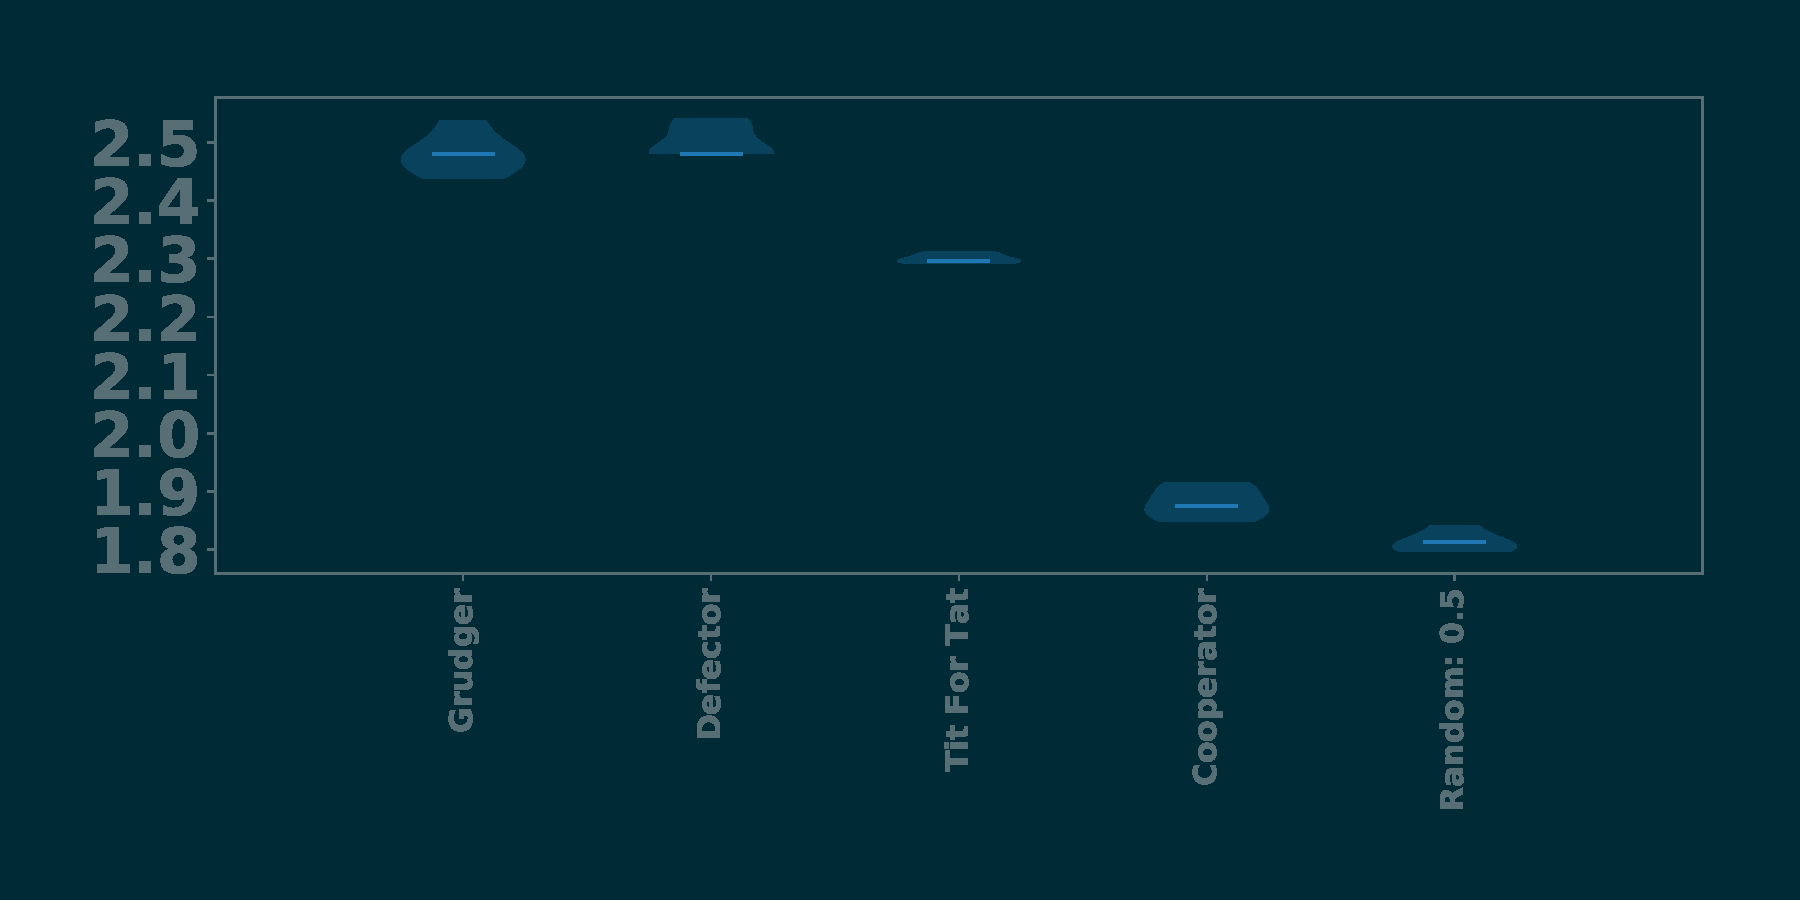
\includegraphics[width=\textwidth, height=0.55\textwidth]{static/tournament_results.pdf}
  \end{column}
      \begin{column}{.30\linewidth}
%%%%%%%%%%%%%%%%%%THIRD QUESTION%%%%%%%%%%%%%%%%%% 
   \vspace{1cm}
   
\begin{center}
        \LARGE{\textcolor{cyan}{SHOULD THE NORTH JOIN HANDS WITH THE SOUTH TO DEFEAT THE NIGHT KING?}} 
        % \\
        % \large{Evolutionary Game Theory allow us to study such population dynamics} 

\vspace{1cm}

\end{center}
        \begin{center}
        \includestandalone[width=0.8\textwidth]{static/evolution}
        \end{center}
    \begin{center}
    \begin{minted}
    [
    autogobble=true,          
    frame=lines,
    framesep=2mm,
    fontsize=\small
    ]
    {python}
import random

N = 5
players = []
axl.seed(5)
for _ in range(N):
    player = random.choice([axl.Defector, axl.Cooperator])
    players.append(player())
    
mp = axl.MoranProcess(players=players, turns=200)
mp.play()

[Counter({'Cooperator': 3, 'Defector': 2}),
 Counter({'Cooperator': 3, 'Defector': 2}),
 Counter({'Cooperator': 3, 'Defector': 2}),
 Counter({'Cooperator': 2, 'Defector': 3}),
 Counter({'Cooperator': 2, 'Defector': 3}),
 Counter({'Cooperator': 1, 'Defector': 4}),
 Counter({'Cooperator': 1, 'Defector': 4}),
 Counter({'Cooperator': 1, 'Defector': 4}),
 Counter({'Defector': 5})]
    \end{minted}
    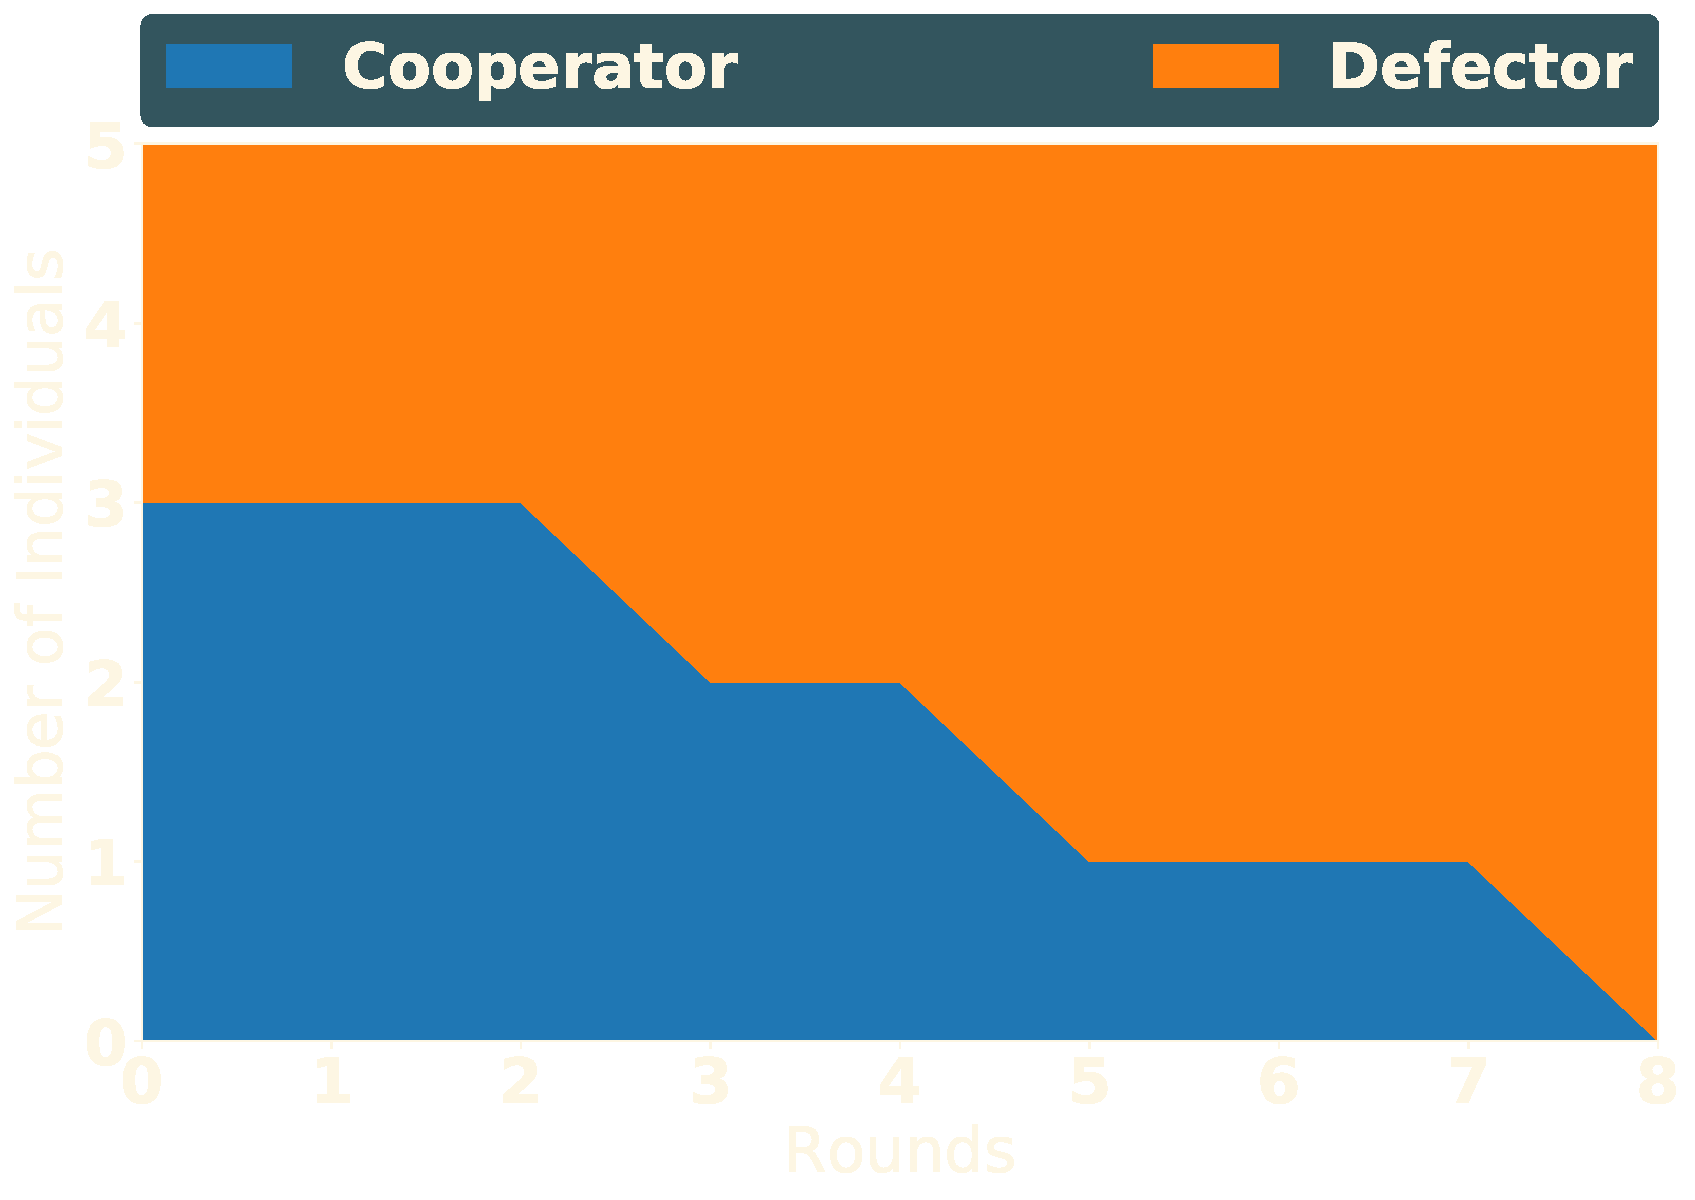
\includegraphics[width=0.7\textwidth, height=0.5\textwidth]{static/evolution_results.pdf}
    \end{center}

    \end{column}
    \end{columns}
\end{frame}
\end{document}
% \noindent\rule[0.5ex]{\linewidth}{1pt}

